\chapter{Maleta de suporte ao abastecimento}

\section{Lista de materiais}

\begin{table}[H]
\centering
\begin{tabular}{|m{2.0cm} |m{9.2cm}|m{2.0cm}|}
\hline
\begin{center}Quantidade\end{center} & \begin{center}Componente\end{center} &\begin{center} Identificador\end{center} \\\hline

    01 & Placa de MDF de 520mm x 330mm x 15mm & 01 \\\hline
    02 & Placa de MDF de 520mm x 300mm x 15mm & 02 \\\hline
    02 & Placa de MDF de 300mm x 300mm x 15mm & 03 \\\hline
    03 & Placa de MDF de 520mm x 165mm x 15mm & 04 \\\hline
    04 & Placa de MDF de 520mm x 70mm x 15mm & 07 \\\hline
    04 & Placa de MDF de 135mm x 70mm x 15mm & 05 \\\hline
    02 & Placa de MDF de 260mm x 165mm x 15mm & 06 \\\hline
    44 & Parafusos cabeça chata M4 x 40mm & 21 \\\hline
    16 & Parafusos cabeça chata M4 x 12mm & 22 \\\hline
    08 & Parafusos de articulação 4mm x 20mm & 24 \\\hline
    20 & Arruelas M5 & 20 \\\hline
    04 & Dobradiças de latão 4 furos 40mm & 08 \\\hline
    02 & Fecho para madeira & 13 \\\hline
    12 & porcas M5 & 18 \\\hline
    02 & dobradiças laterais tipo sanfona & 16 \\\hline
    02 & cilindros de madeira vazado de 200mm de comprimento & 19 \\\hline
    08 & parafusos para os fechos & 23 \\\hline
    08 & parafusos flangeados para dobradiça lateral & 26 \\\hline
    02 & fusos M5 de 540mm de comprimento & 17 \\\hline
    01 & manta SBR de $1 m^2$ & -  \\\hline

\end{tabular}
\label{table: tabelaComponentesMaletaIgnicao}
\caption{Lista de componentes}
\end{table}

\begin{figure} [H]
    \centering
    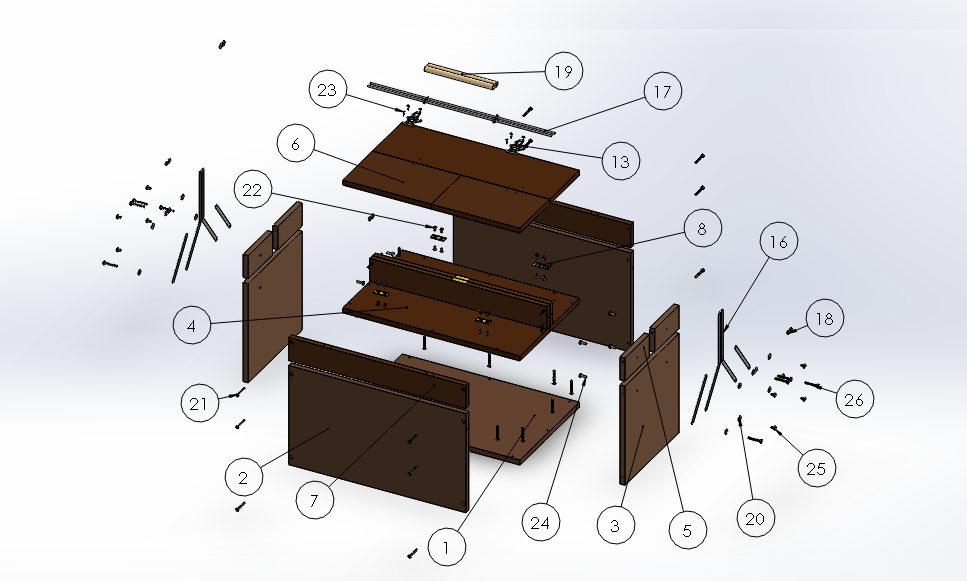
\includegraphics[width=\textwidth]{Figuras/montagemMaletasEstrutura/ignicaoExplodida.png}
    \caption{Visão explodida da maleta do sistema de alimentação}
    \label{fig:ignicaoExplodida}
\end{figure}



\section{Ferramentas}

\par Para a montagem da estrutura da maleta:
\begin{itemize}
    \item Furadeira
    \item Broca padrão de 2mm
    \item Broca para madeira de 3mm
    \item Punção
    \item Parafusadeira E conjunto de chaves \textit{Philips}
    \item Trena
\end{itemize}
\par Para a fixação do revestimento:
\begin{itemize}
    \item estilete
    \item pistola de cola quente
\end{itemize}

\section{Fabricação da estrutura}
\subsubsection{Chapa de MDF}
 As chapas de MDF são vendidas normalmente em tamanhos pré-definidos, geralmente de grandes dimensões (2750mm x 1840mm). Porém, é praxe as lojas oferecerem o serviço, que pode ser cobrado à parte, de corte da chapa no tamanho que o cliente deseja. Portanto, é bom já com as dimensões das peças com as quais pretende trabalhar na hora da compra, que o vendedor elaborará um plano de corte para a chapa a ser adquirida.
    \par É comum a quantidade total de peças desejada não ocupar totalmente a área padrão da chapa vendida, sobrando rebarbas, ou necessitando adquirir uma chapa extra para uma única peça que não coube junto com as outras na chapa original. Cabe ao projetista avaliar se seu projeto permite um redimensionamento das peças para otimização do plano de corte, ou se a economia de material não compensa esse tipo de modificação.
\subsubsection{Peças metálicas}
Quanto aos metais utilizados, apenas as dobradiças laterais, que dão o suporte à alça, precisam ser fabricadas. Elas são peças planas, de desenho relativamente simples (cf.\ref{fig:dobradicaLateral}, dimensões encontram-se no desenho técnico em apêndice) e corte perpendicular, logo o uso de uma máquina de Comando Numérico Computadorizado (CNC) certamente será suficiente para a fabricação das peças. Recomenda-se trabalhar com aço, uma vez que a alça receberá a carga do peso da maleta.

\subsubsection{Revestimento SBR}

Caso se opte por revestir as maletas com borracha SBR, realizar sua fixação com  o uso de cola quente. Importante observar se a manta está fixada em todas as arestas, de modo a não ter entrada de água ou outro tipo de material indesejado na interface entre o revestimento e a face do MDF. É possível fixar acabamentos metálicos nas arestas da maleta, de modo a reforçar a fixação do revestimento, ou mesmo evitar que este se descole a partir de uma de suas bordas.
Usar estilete para acabamento fino, principalmente em torno das peças metálicas, como o fecho e as dobradiças.

\begin{figure}[H]
    \centering
    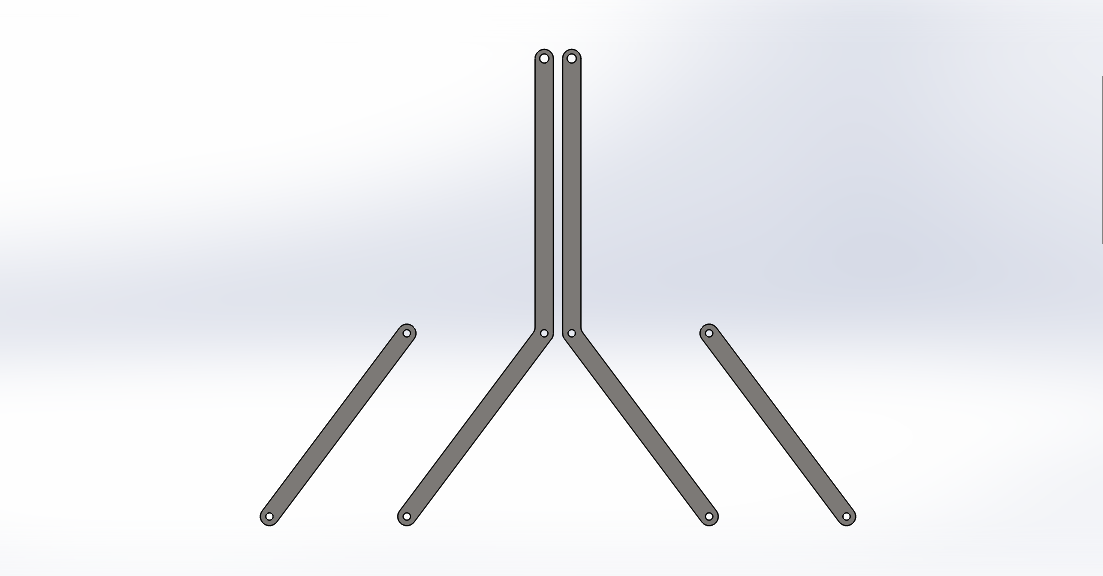
\includegraphics[width=.7\textwidth]{Figuras/montagemMaletasEstrutura/alimentacaoDobradicaLateral.png}
    \caption{Desenho das dobradiças laterais, que dão suporte às alças}
    \label{fig:dobradicaLateral}
\end{figure}

\section{Fixação dos componentes}

\subsection{Preparação dos furos}

   \par Antes de iniciar a montagem das peças, é importante estabelecer algumas regras sobre a criação dos furos e a fixação dos parafusos que serão válidas para todos os casos, independentemente de suas posições:
    \begin{enumerate}
        \item Como regra geral, os parafusos de 40mm serão usados nos furos perpendiculares à chapa. Entende-se como perpendicular o furo criado na face da espessura (15mm) da peça, ou, em outras palavras, os furos que estejam no mesmo sentido das fibras do MDF;
        \item Os furos perpendiculares sempre estarão a 7,5mm de distância de sua aresta mais próxima, mesmo que não haja indicação dessa distância. Assim, garante-se que o parafuso seja fixado no centro da espessura da peça;
        \item A disposição dos furos é simétrica. Mesmo que o desenho não mostre a disposição dos furos na face oposta àquela que está em destaque, pressupõe-se que essa disposição segue a simetria no plano vertical (eixos de simetria são indicados para auxiliar a visualização).
        
\end{enumerate}
  
  \begin{figure} [H]
    \centering
    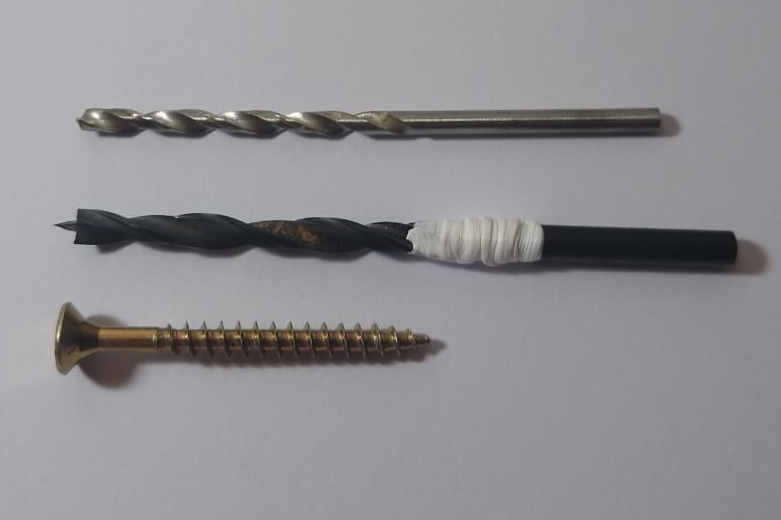
\includegraphics[width=.7\textwidth]{Figuras/montagemMaletasEstrutura/brocas.png}
    \caption{Brocas de 2mm e 3mm para preparação do furo}
    \label{fig:brocas1}
\end{figure}
  
\par Os furos reservados para os parafusos de 40mm seguirão o seguinte protocolo:

\begin{enumerate}
    \item Marcar o local dos furos na chapa (conforme indicação a seguir) com o uso da punção e uma trena;
    \item Fazer um furo guia com a furadeira e a broca de 2mm de diâmetro. Cuidado para que o furo seja perpendicular à superfície que se está furando;
    \item Fazer furo o definitivo com a broca para madeira de 3mm. O diâmetro do furo deve ser menor que o do parafuso para que a rosca se fixe nas fibras da madeira;
    \item Como os parafusos de 40mm serão fixados no sentido perpendicular, a profundidade do furo não é de grande preocupação. Porém, como veremos no esquema de montagem, alguns parafusos ficam próximos um do outro. Ainda que a disposição dos furos tenha sido pensada para que haja uma boa margem de distância entre esses parafusos, é bom ficar atento, principalmente se a montagem estiver sendo feito de maneira intercalada (furo - parafuso - furo - parafuso - ...). Uma dica é marcar a broca com uma fita adesiva usando o parafuso de referência como na figura \ref{fig:brocas1}. Cuidado para a fita não interferir na fixação da broca no bocal da furadeira.
    \item Quanto aos parafusos de 12mm, não é necessário fazer furo prévio. Marcar com a punção e parafusar direto com a parafusadeira já é suficiente.
\end{enumerate}

\subsection{Esquema de montagem}

A seguir, serão mostradas uma série de imagens mostrando a sequência de montagem de cada peça da maleta do sistema de ignição. As imagens são apenas para ilustrar o passo a passo da fixação dos parafusos, e a ordem recomendada para a montagem, da parte inferior, passando pelas duas partes superiores, os tampos, dobradiças, fecho e alça. A posição dos parafusos encontra-se no fim desta seção.

\subsubsection{Montagem da parte inferior}

Materiais utilizados: 1 peça (01), 2 peças (02), 2 peças (03) e 14 parafusos (21).

\begin{figure} [H]
    \centering
    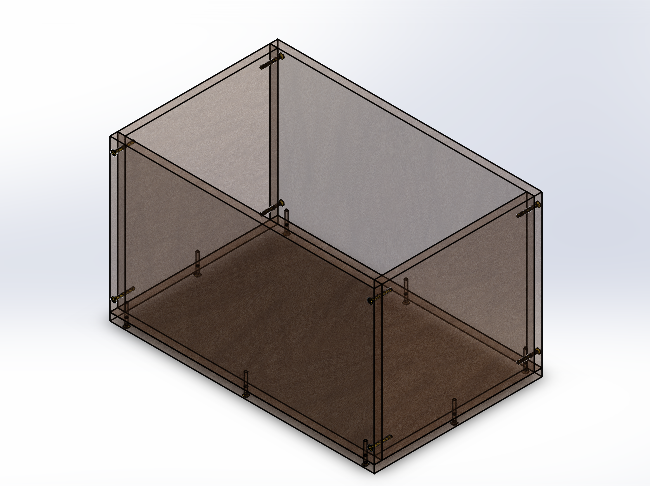
\includegraphics[width=.7\textwidth]{Figuras/montagemMaletasEstrutura/alimentacaoBase.png}
    \caption{Posição dos parafusos da parte inferior}
    \label{fig:alimentacaoBase}
\end{figure}

\begin{figure} [H]
    \centering
    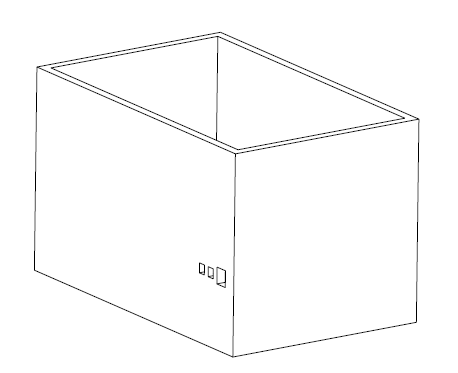
\includegraphics[width=.5\textwidth]{Figuras/suporte/base.png}
    \caption{Base}
\end{figure}

\subsubsection{Montagem das partes superiores}

Materiais utilizados: 2 peças (04), 4 peças (05) 4 peças (07) e 28 parafusos (21).

\begin{figure} [H]
    \centering
    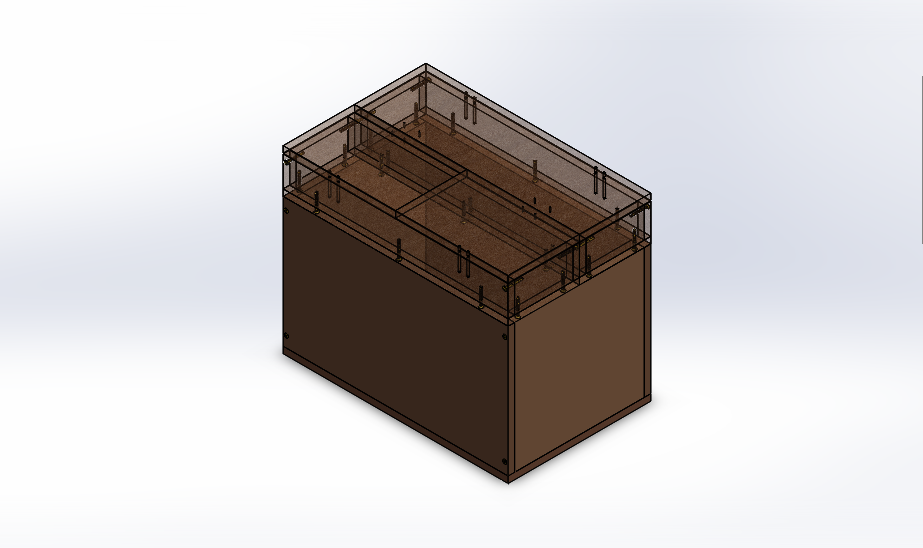
\includegraphics[width=.7\textwidth]{Figuras/montagemMaletasEstrutura/alimentacaoGavetas.png}
    \caption{Posição dos parafusos das partes superiores}
    \label{fig:alimentacaoGavetas}
\end{figure}

\begin{figure} [H]
    \centering
    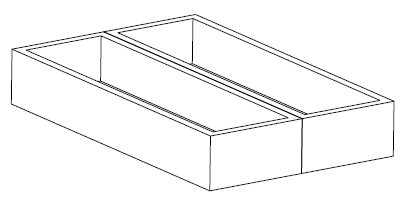
\includegraphics[width=.5\textwidth]{Figuras/suporte/laterais.png}
    \caption{Base das laterais}
\end{figure}

\subsubsection{Montagem dos tampos e dobradiças}

Materiais utilizados: 1 peça (04), 2 peças (06), 2 dobradiças (08), 4 parafusos (21) e 4 parafusos (22).
\par O tampo da maleta é formado por três peças, uma maior e duas menores, de metade do comprimento do tampo maior, de forma ao usuário ter acesso independente a cada uma das áreas da gaveta que leva o sistema válvula + motor. Para manter a simetria, a dobradiça deve ser fixada no meio desses tampos menores, e na mesma posição equivalente no tampo maior, conforme indica a distância na ilustração. Atentar-se para a escolha dos parafusos: os de 40mm vão nos furos longitudinais (furos da parede), e os de 12mm vão nos furos transversais (furo do tampo). 

\begin{figure} [H]
    \centering
    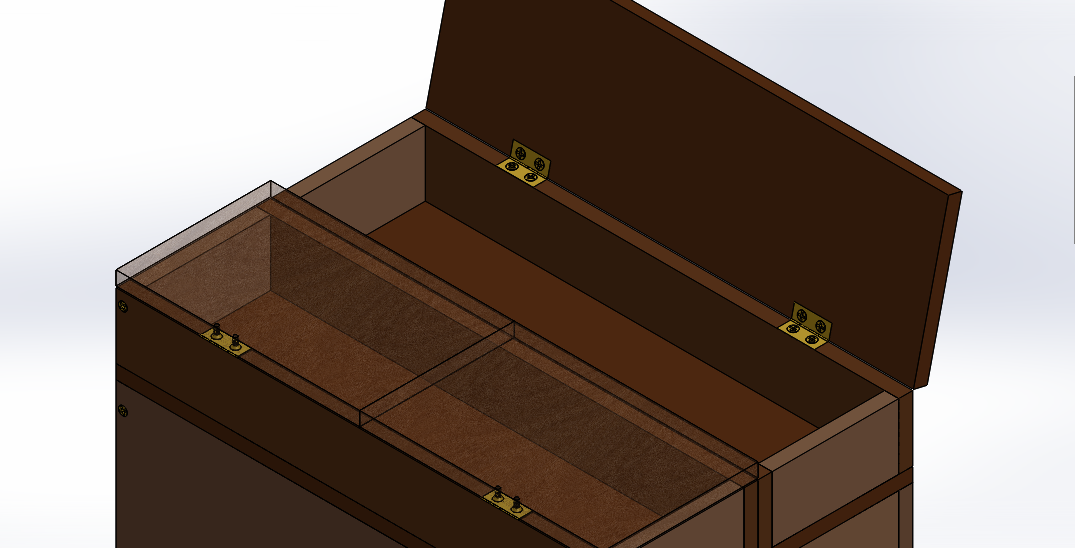
\includegraphics[width=.7\textwidth]{Figuras/montagemMaletasEstrutura/alimentacaoDobradicas.png}
    \caption{Montagem das dobradiças na lateral e no tampo da maleta}
    \label{fig:alimentacaoDobradicas}
\end{figure}

\begin{figure} [H]
    \centering
    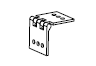
\includegraphics[width=.5\textwidth]{Figuras/suporte/dobradicas.png}
    \caption{Dobradiças}
\end{figure}

\begin{figure} [H]
    \centering
    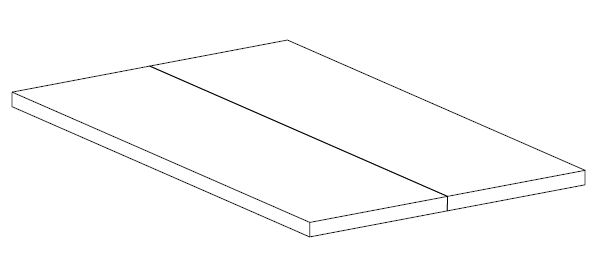
\includegraphics[width=.7\textwidth]{Figuras/suporte/tampas.png}
    \caption{Tampas}
\end{figure}

\subsubsection{Montagem dos fechos}

Materiais utilizados: 2 fechos (13) e 8 parafusos (23).

\par Esse é o passo da montagem mais passível de mudança. Ao mesmo tempo, é o que menos afeta o funcionamento correto da maleta, uma vez que o fecho não receberá carga em seu uso recorrente. Os tipos de fecho encontrados comercialmente podem variar um pouco as suas dimensões, o que afeta a posição de seus furos, ou até mesmo a dimensão deles, podendo-se necessitar de parafusos de diâmetros menores que os utilizados nesse projeto. Como regra geral, recomenda-se manter a simetria ilustrada na figura \ref{fig:fechos},  principalmente em relação aos tampos menores.

\begin{figure}[H]
    \centering
    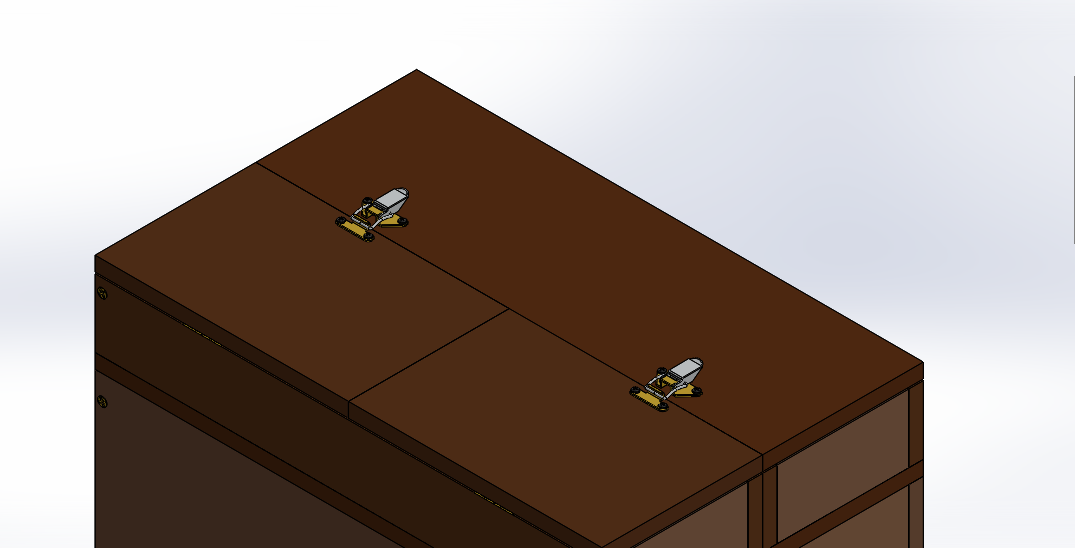
\includegraphics[width=.7\textwidth]{Figuras/montagemMaletasEstrutura/alimentacaoFechos.png}
    \caption{Montagem dos fechos nos tampos da maleta}
    \label{fig:fechos}
\end{figure}

\begin{figure} [H]
    \centering
    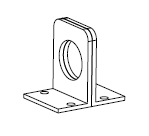
\includegraphics[width=.5\textwidth]{Figuras/suporte/trancas.png}
    \caption{Trancas}
\end{figure}

\subsubsection{Montagem da alça com as dobradiças laterais}

Materiais utilizados: 8 parafusos (26), 8 parafusos (24), 20 arruelas (20), 1 conjunto de dobradiças laterais (16), 2 fusos (17) e 12 porcas (18).

A última etapa da montagem envolve uma fixação diferente das outras que foram feitas, por se tratar de uma parte móvel. Para tanto, não será possível utilizar o parafuso de 12mm para os furos transversais da \ref{fig:ignicaoAlca}. No lugar deles, utilizaremos um parafuso para articulação do tipo união (cf. \ref{fig:parafusoUniao}) em um furo trespassado. A fixação do parafuso união por ambos os lados demandará que uma de suas cabeças seja segurada com uma chave \textit{Philips} enquanto o outro lado é rosqueado por outra chave ou pela furadeira.

\begin{figure}[H]
    \centering
    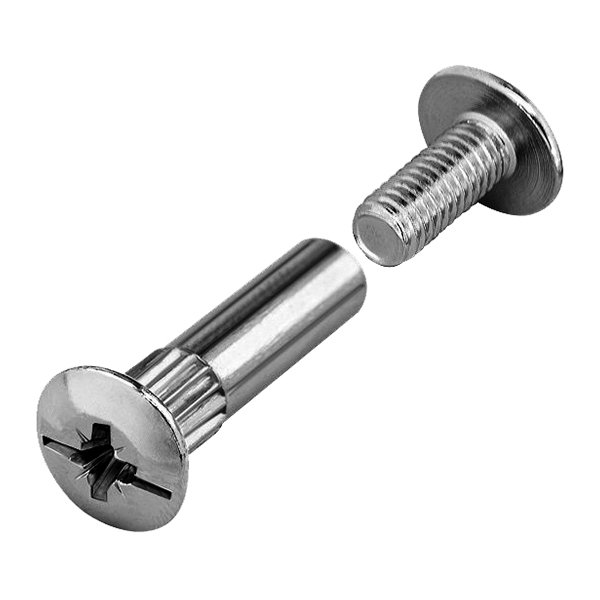
\includegraphics[width=.3\textwidth]{Figuras/montagemMaletasEstrutura/parafusoUniao.jpg}
    \caption{Parafuso para articulação das alças laterais}
    \label{fig:parafusoUniao}
\end{figure}

\begin{figure} [H]
    \centering
    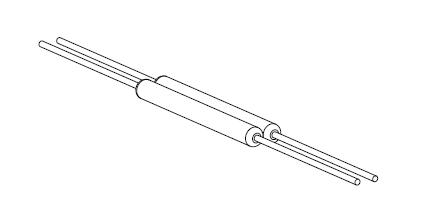
\includegraphics[width=.5\textwidth]{Figuras/suporte/alcas.png}
    \caption{Alças}
\end{figure}

\begin{figure} [H]
    \centering
    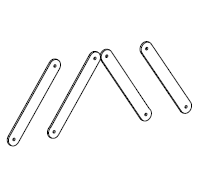
\includegraphics[width=.5\textwidth]{Figuras/suporte/dobradicas_laterais.png}
    \caption{Dobradiças Laterais}
\end{figure}

\par Mas antes disso, vamos para a montagem da alça em si: passa-se o furo pelo cilindro de madeira, que servirá de empunhadura para a maleta. Em seguida, passam as arruelas, que servirão de interface entre a madeira e as porcas que fixarão a empunhadura no meio do fuso. por fim para mais um conjunto de porcas, que servirá para fixar o fuso nos furos superiores das alças laterais. Coloca-se, por fim mais duas porcas, uma em cada lado, para fazer a fixagem final da alça.

\begin{figure}[H]
    \centering
    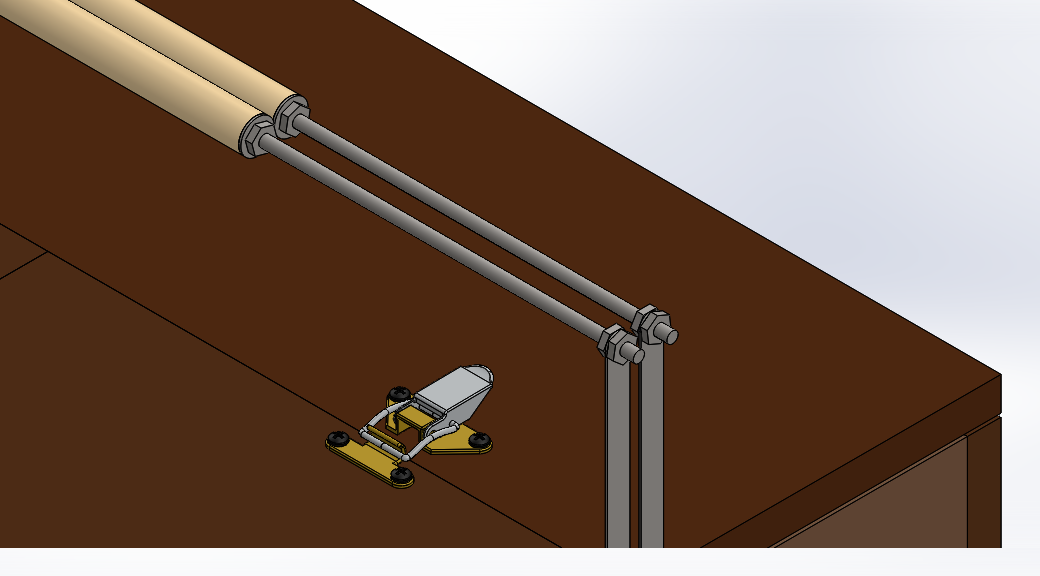
\includegraphics[width=.7\textwidth]{Figuras/montagemMaletasEstrutura/alimentacaoAlcaDetalhe.png}
    \caption{Detalhe da montagem da alça e sua fixação nas dobradiças laterais}
    \label{fig:parafusoUniao}
\end{figure}

\par Fixamos por fim a alça recém-montada nos furos laterais da maleta. Utilizaremos uma arruela em cada um dos parafusos que fixam a alça, de modo a criar um espaço entre o suporte da alça e a parede lateral da maleta. Quanto aos furos longitudinais (aqueles que vão no sentido da fibra longitudinalmente à chapa de MDF), continuaremos utilizando os parafusos de 40mm, uma vez que os parafusos da alça receberão a carga do peso da maleta. Porém esses furos terão a cabeça flangeada, em vez de cônica como as que usamos para a madeira, uma vez que a cabeça desses parafusos estará em contato com o metal das dobradiças, cujos furos não terão aquele acabamento cônico dos furos em madeira. Além disso, esses parafusos devem deixar uma folga no seu aperto, de modo a permitir que as dobradiças laterais rotacionem livremente. Fixados esses últimos parafusos, a estrutura da maleta estará pronta.
 

\begin{figure}[H]
    \centering
    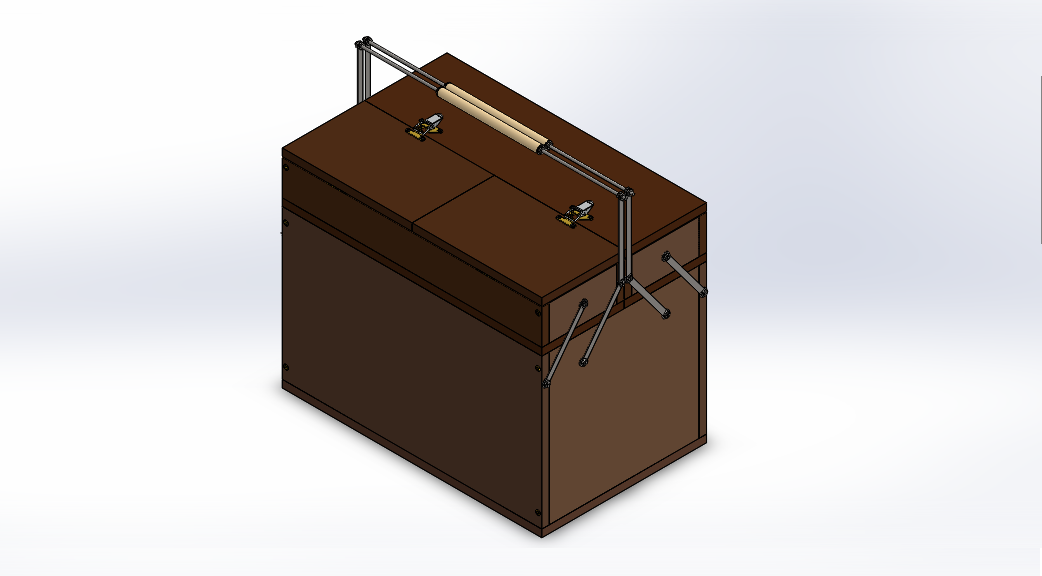
\includegraphics[width=.7\textwidth]{Figuras/montagemMaletasEstrutura/alimentacaoMontada.png}
    \caption{Montagem final da maleta do sistema de alimentação}
    \label{fig:ignicaoAlca}
\end{figure}

\subsubsection{Revestimento}

Caso se opte por revestir as maletas com borracha SBR, realizar sua fixação com  o uso de cola quente. Importante observar se a manta está fixada em todas as arestas, de modo a não ter entrada de água ou outro tipo de material indesejado na interface entre o revestimento e a face do MDF. É possível fixar acabamentos metálicos nas arestas da maleta, de modo a reforçar a fixação do revestimento, ou mesmo evitar que este se descole a partir de uma de suas bordas.

\begin{figure} [H]
    \centering
    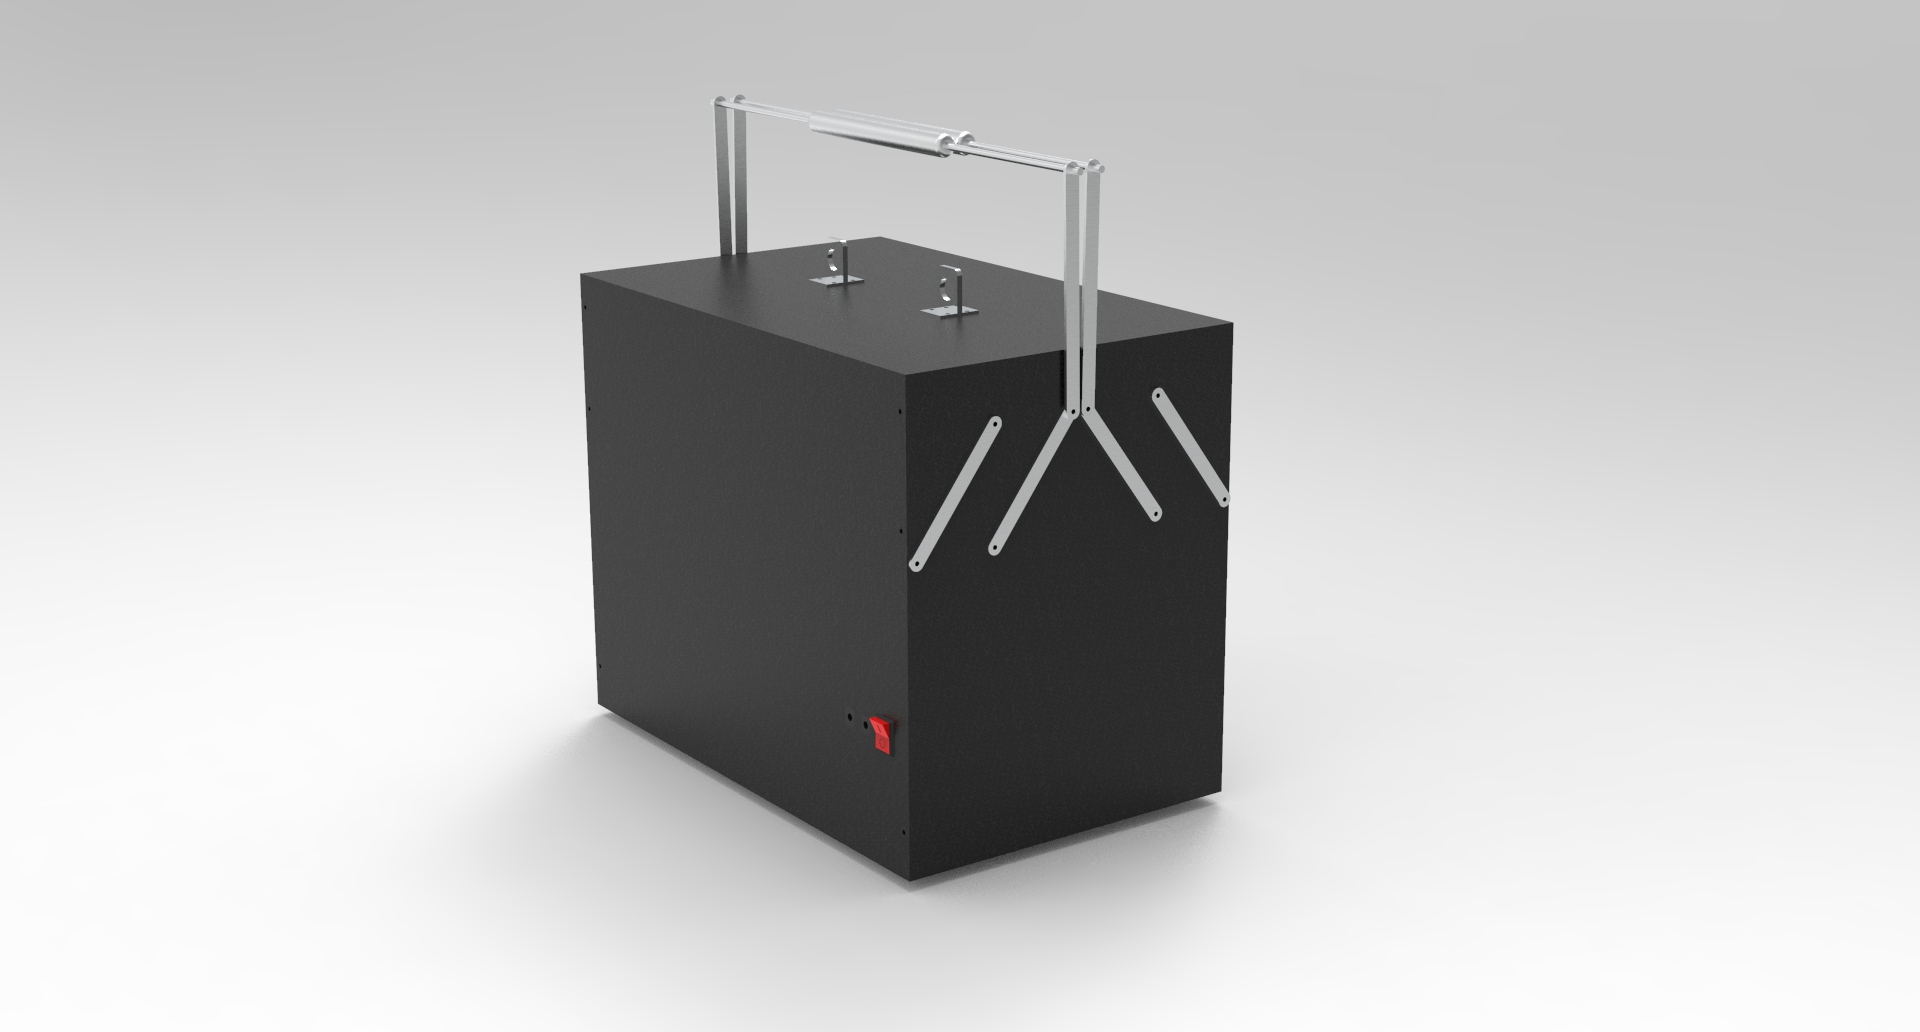
\includegraphics[width=.5\textwidth]{Figuras/suporte/untitled.4.jpg}
    \caption{Montagem final da maleta do sistema de alimentação com revestimento fechada}
\end{figure}

\begin{figure} [H]
    \centering
    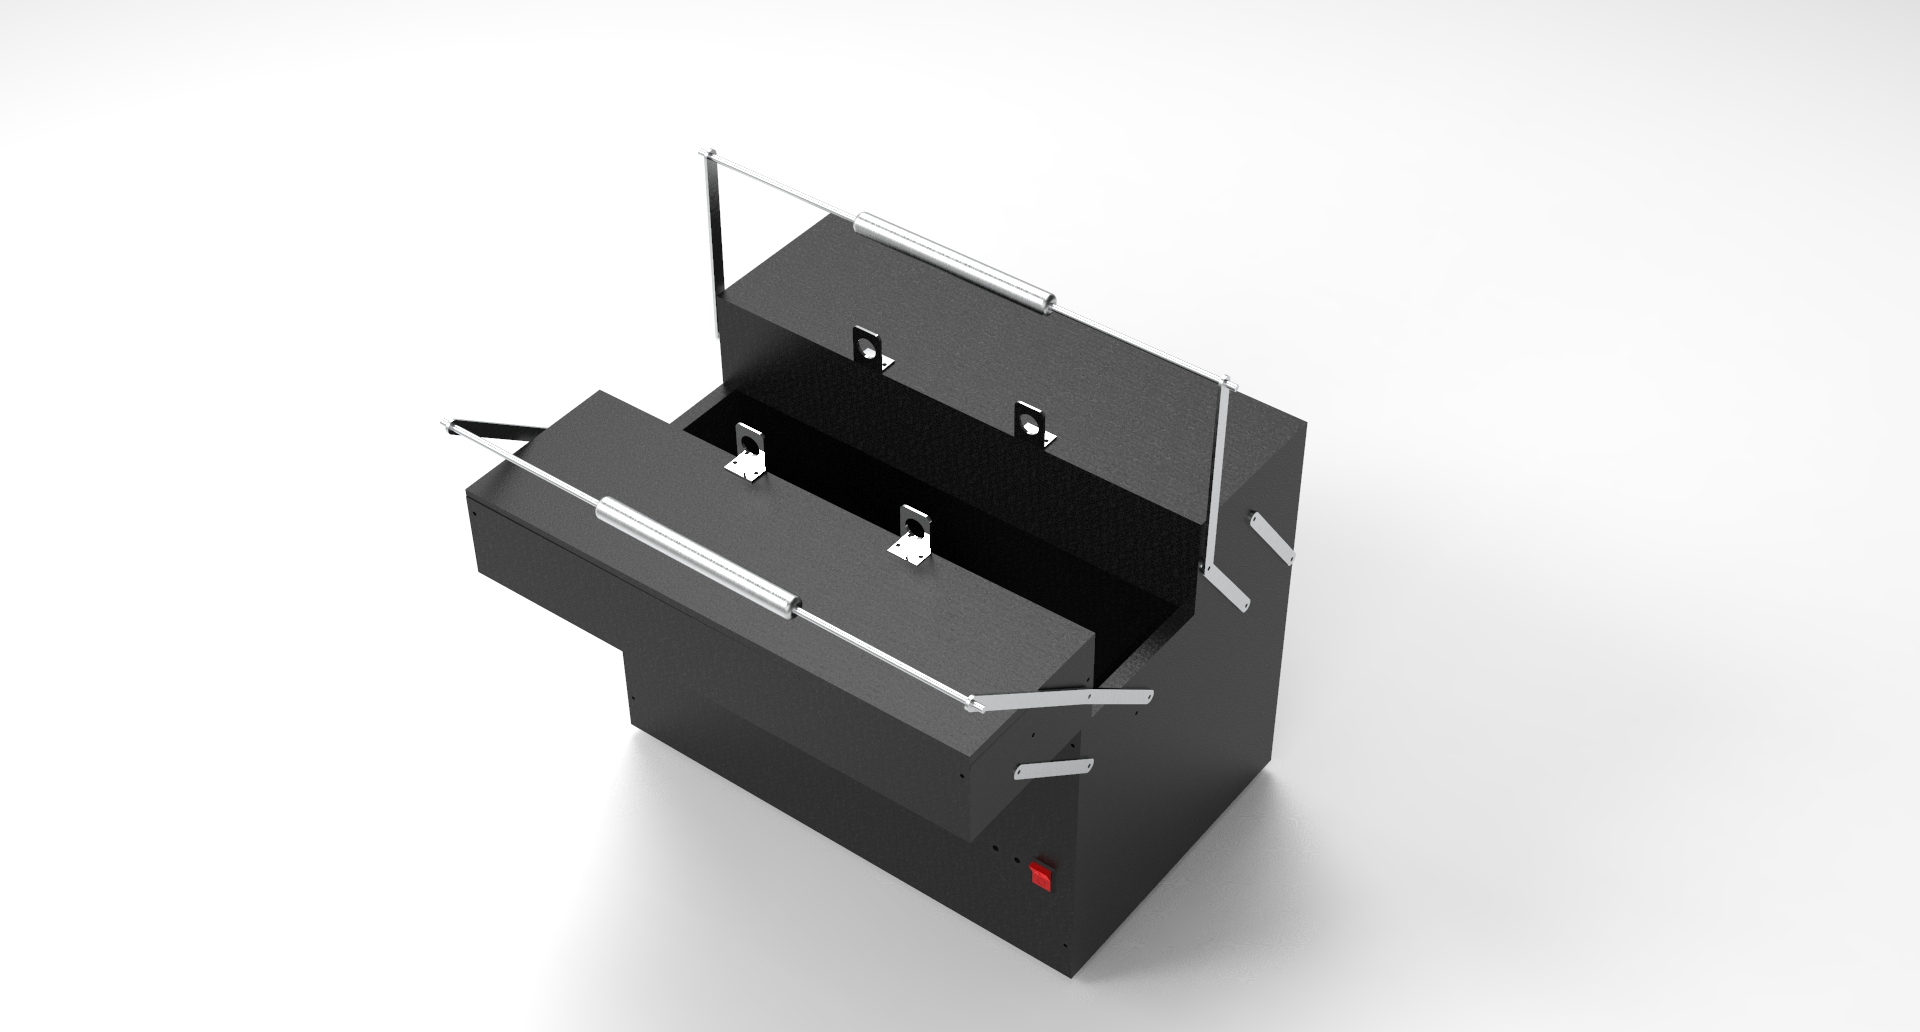
\includegraphics[width=.5\textwidth]{Figuras/suporte/untitled.5.jpg}
    \caption{Montagem final da maleta do sistema de alimentação com revestimento aberta}
\end{figure}

\subsubsection{Posição dos furos}

\begin{figure}[H]
    \centering
    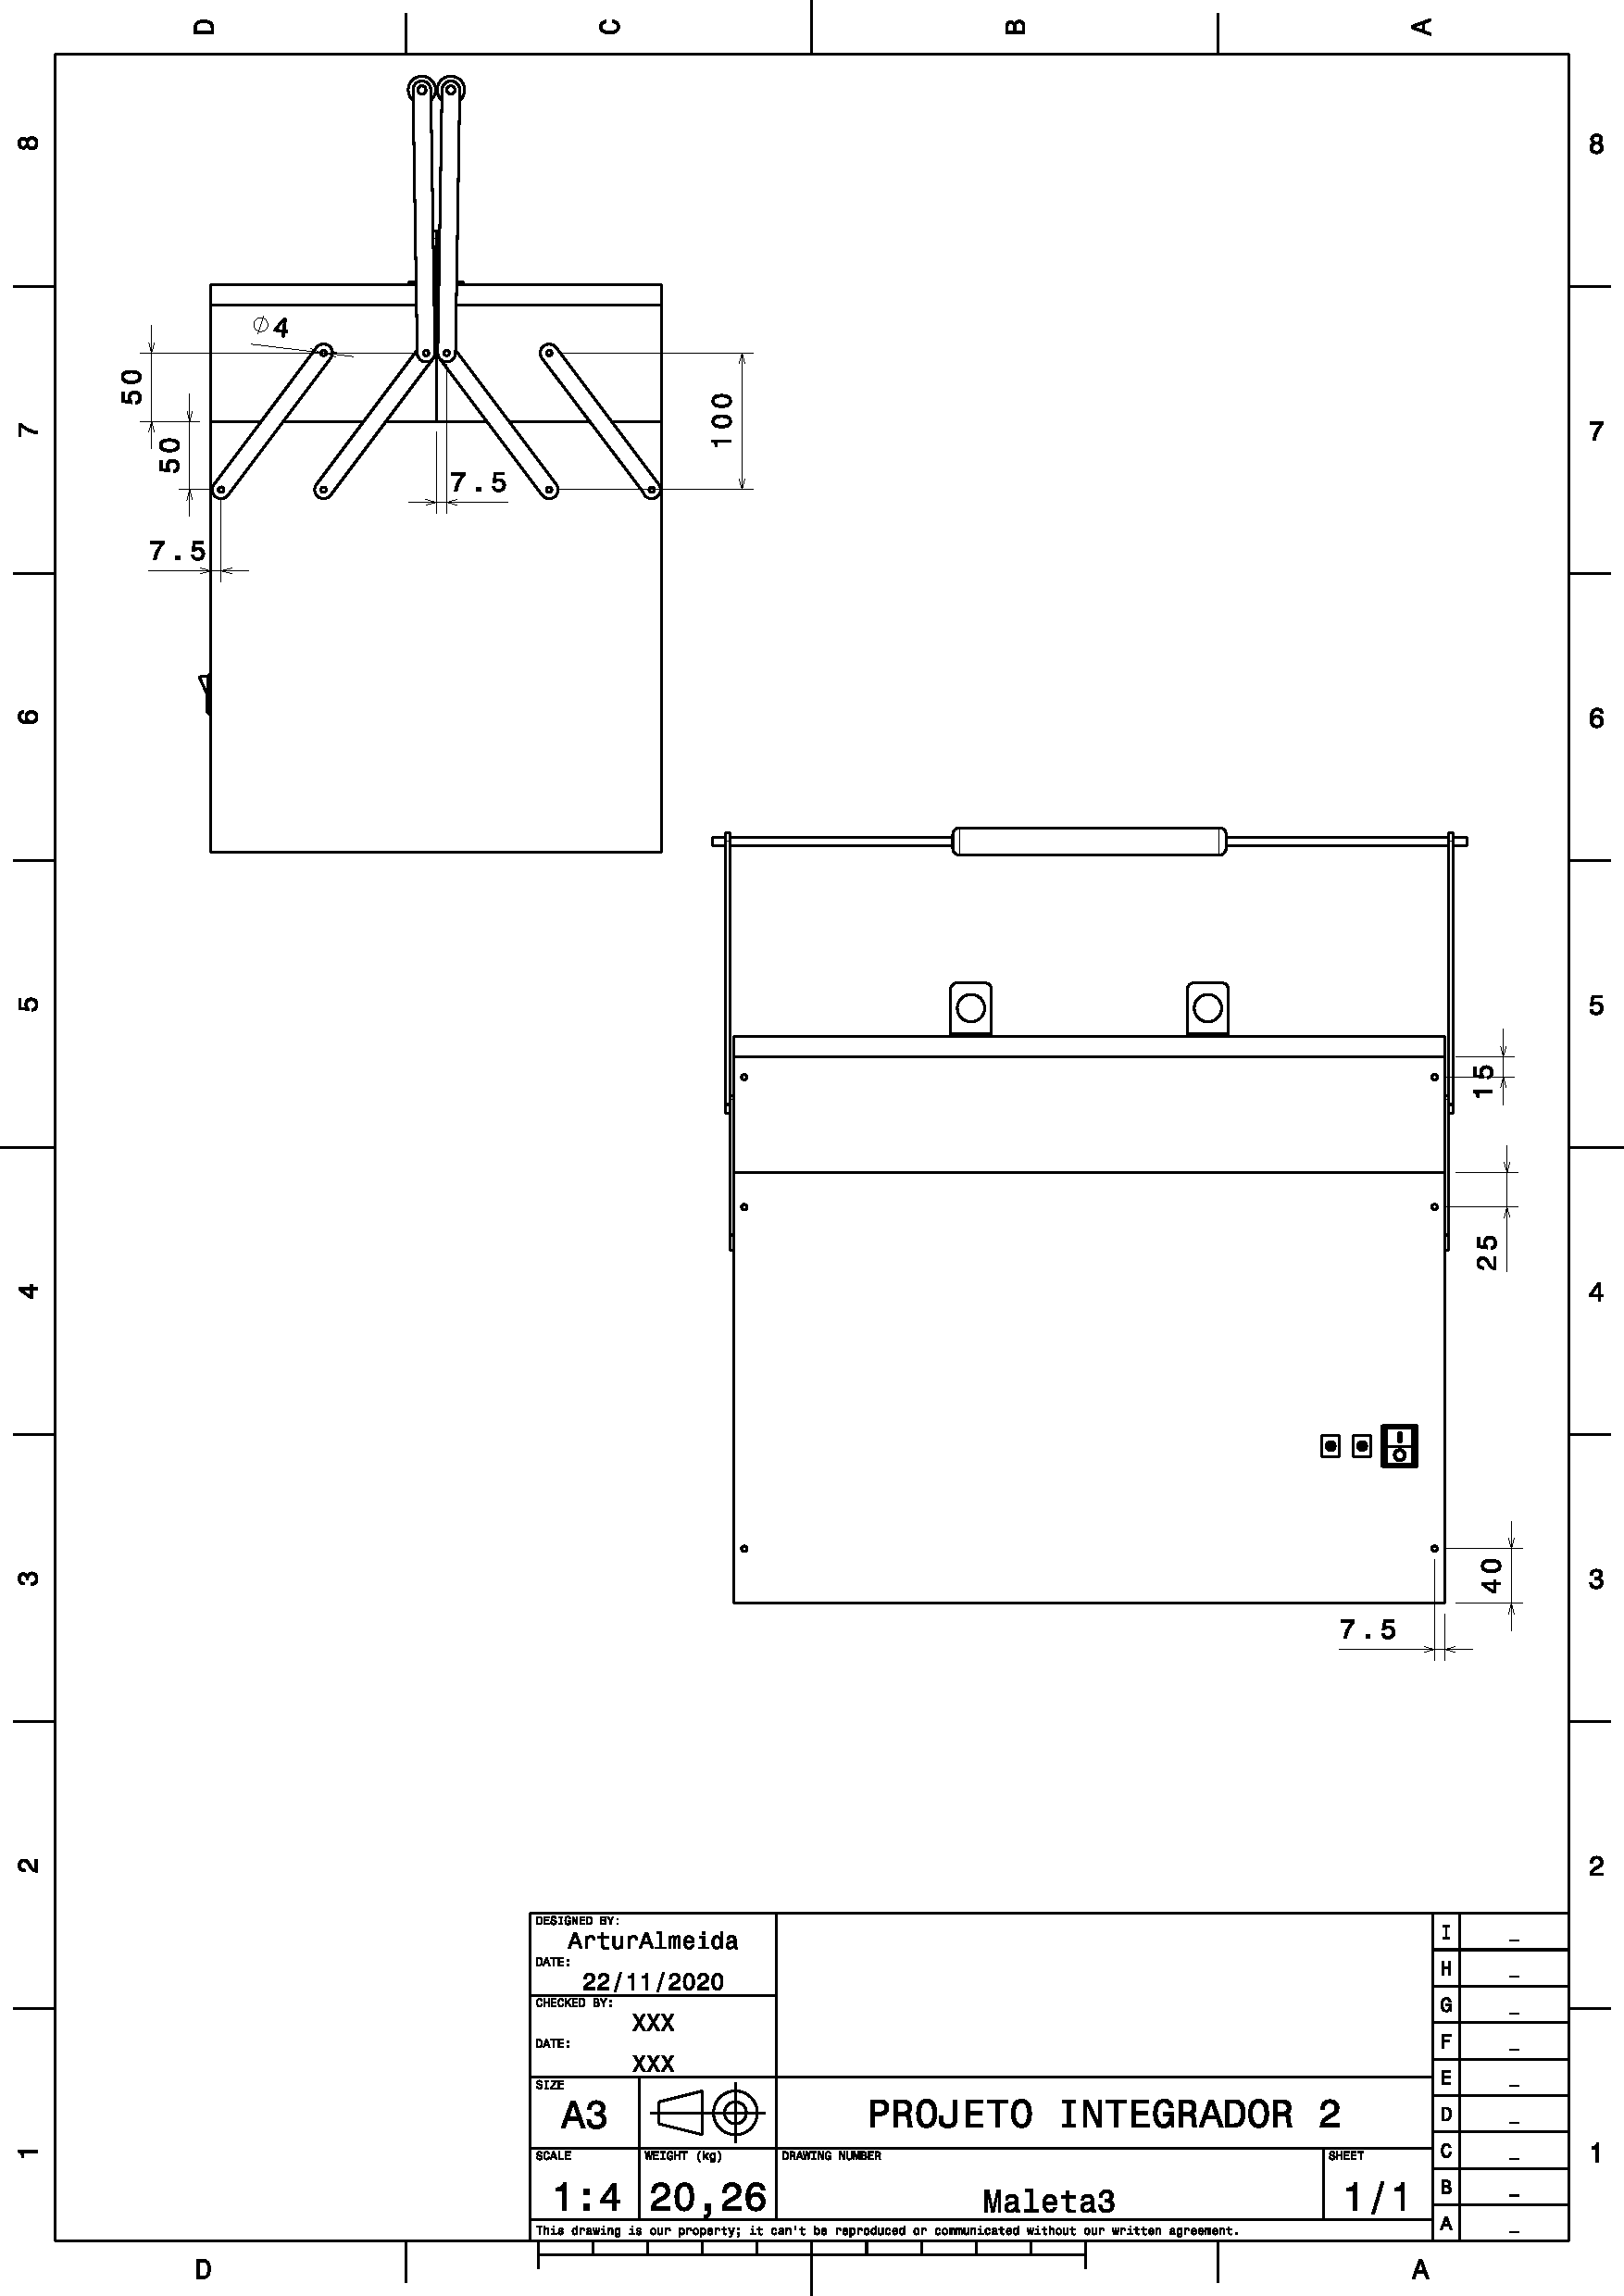
\includegraphics[width=.7\textwidth]{Figuras/montagemMaletasEstrutura/PARAFUSOALIMENTAÇÃO1.pdf}
    \caption{Vista lateral da posição dos furos}
    \label{fig:posicaoFuroAlimentacao1}
\end{figure}

\begin{figure}[H]
    \centering
    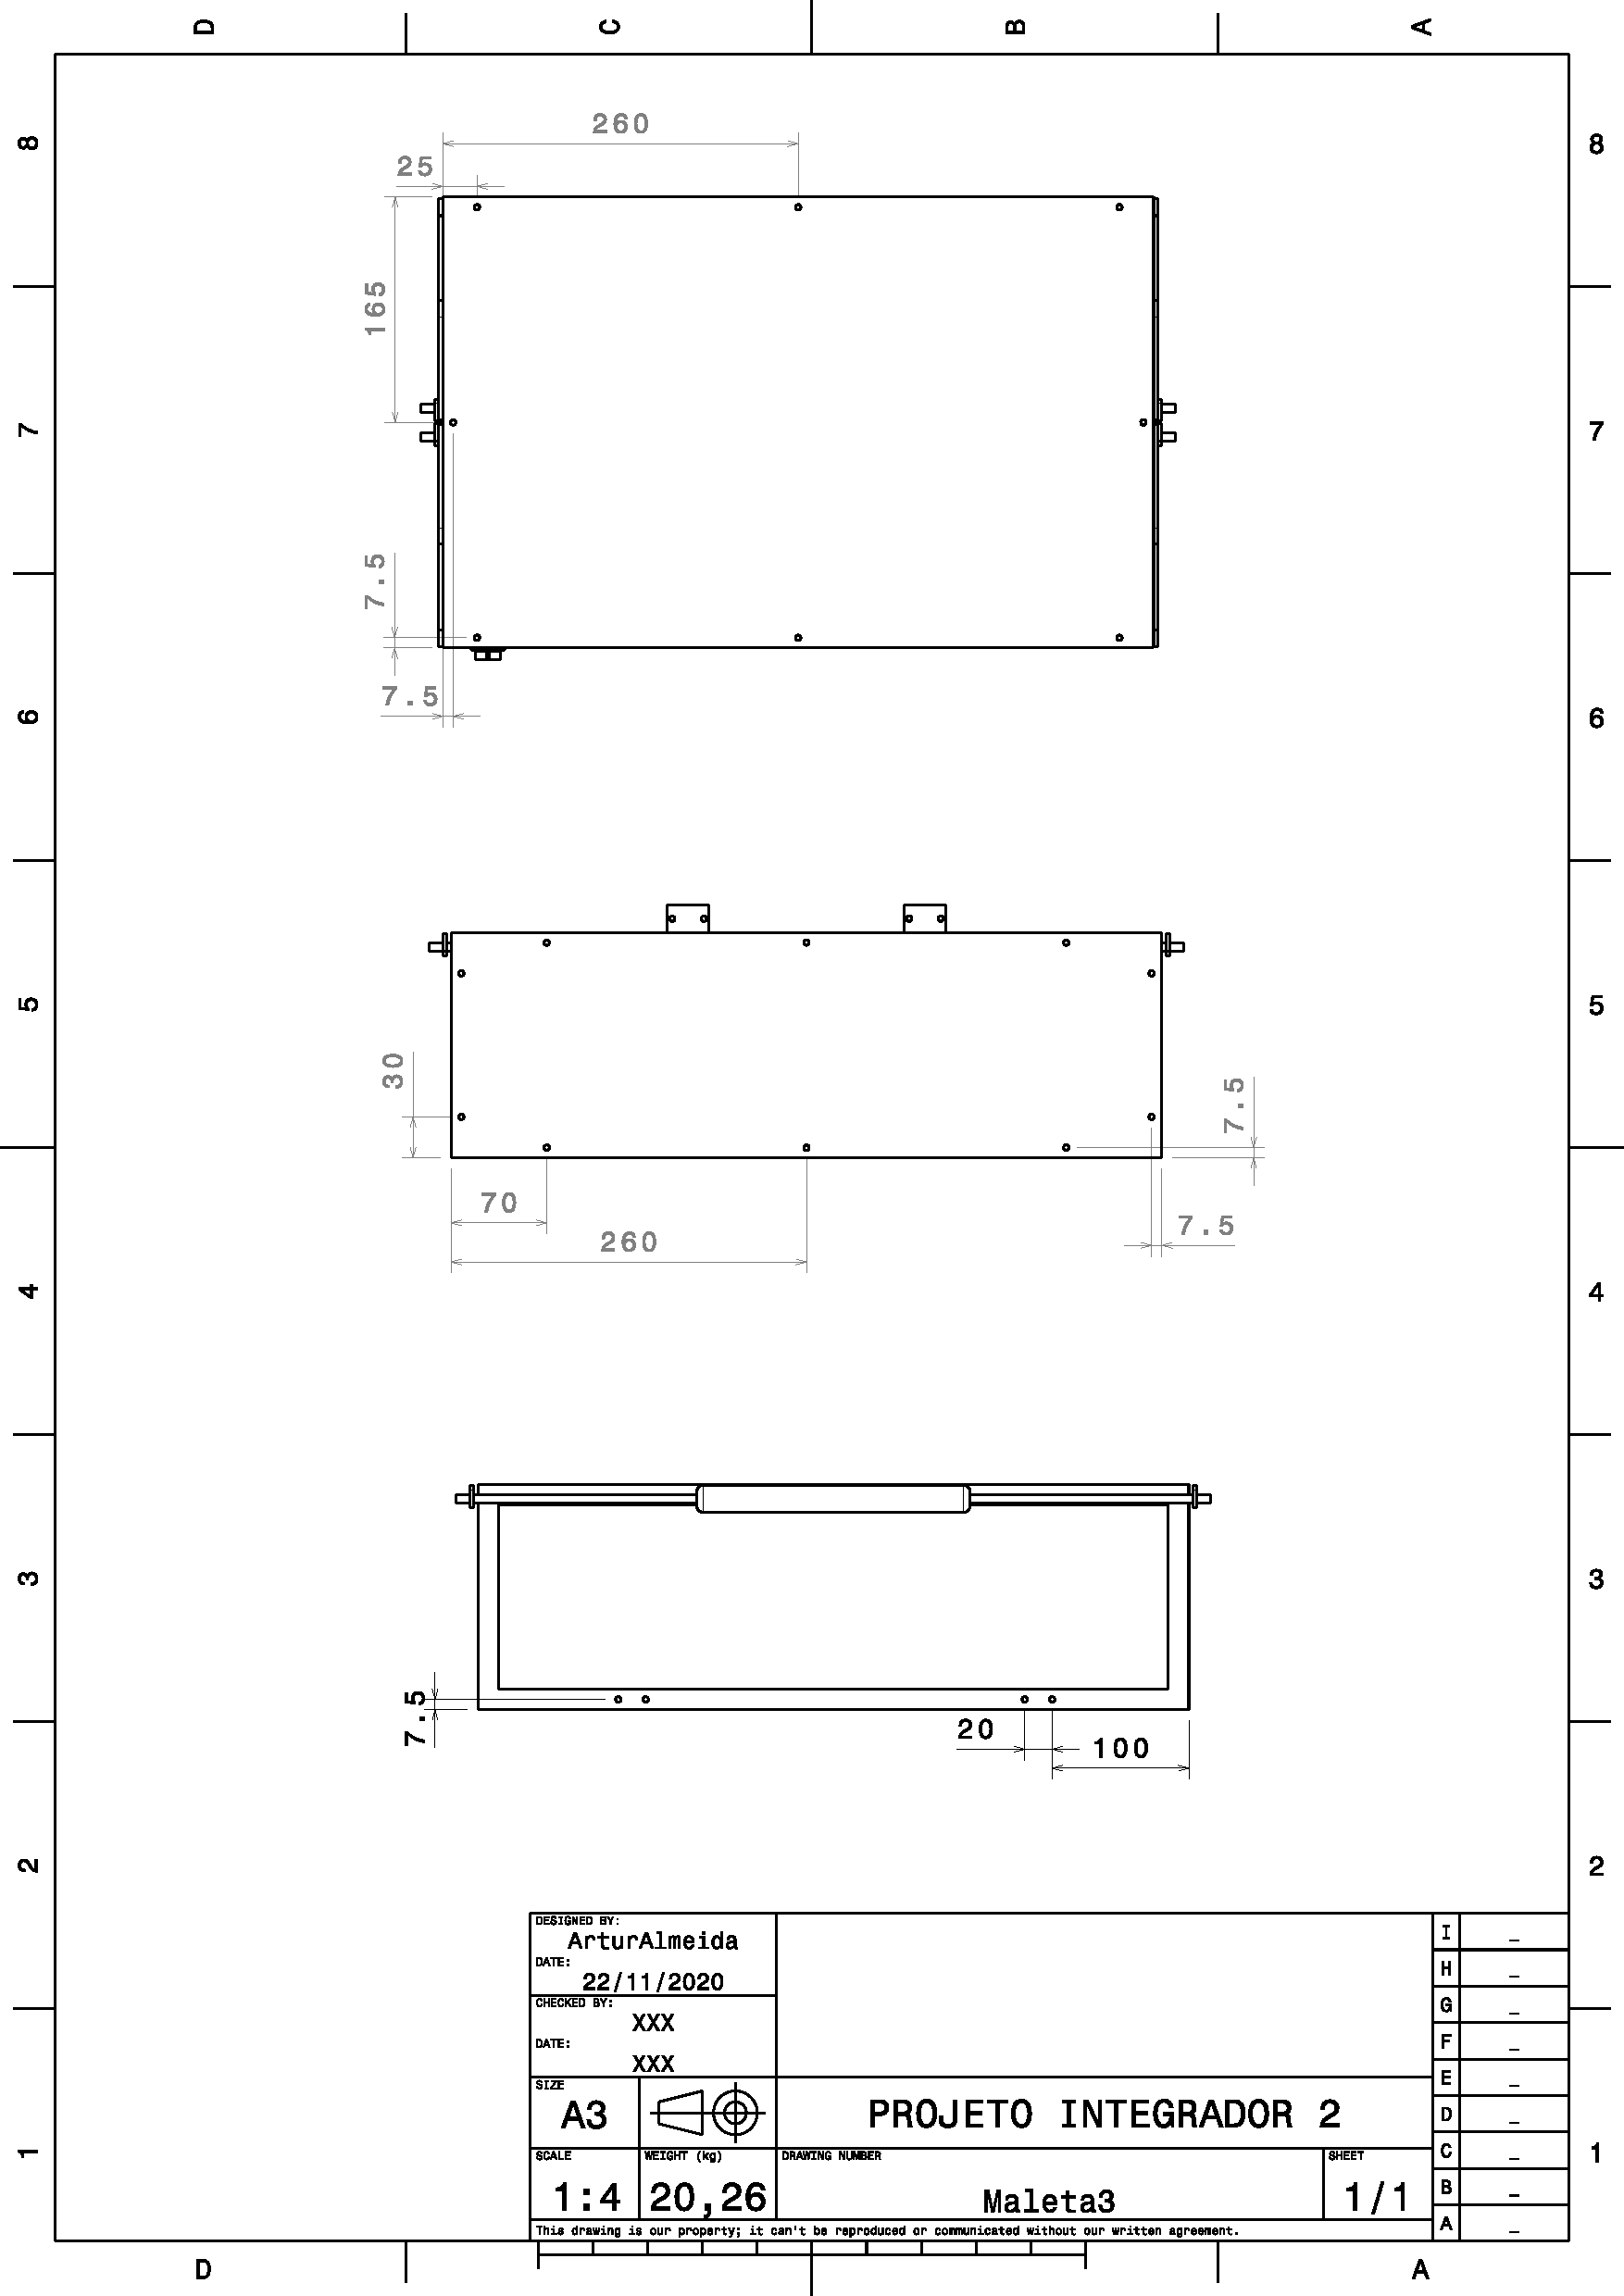
\includegraphics[width=\textwidth]{Figuras/montagemMaletasEstrutura/PARAFUSOALIMENTAÇÃO2.pdf}
    \caption{Vista superior da posição dos furos}
    \label{fig:posicaoFuroAlimentacao2}
\end{figure}

\section{Conexões do sistema de alimentação}

Antes de iniciar a montagem do sistema de alimentação se atentar as orientações contidas no Plano de Teste deste manual.

\subsection*{Lista de materiais}

\begin{table}[H]
\centering
\begin{tabular}{|m{1.8cm} |m{9.2cm}|m{4cm}|}
\hline
\begin{center}Quantidade\end{center} & \begin{center}Componente\end{center} &\begin{center} Part Number\end{center} \\\hline
 03&Conectores Jack J4 DC femea& Jack fêmea \\\hline
 01 & Bateria Lítio 12V 10Ah UPLFP12-10 & UPLFP12-10 \\\hline
 02 & Kits 2 Garra Jacaré média (01 Vermelha E 01 Preta) - 20A & - \\\hline
 01 & Chave Gangorra KCD4-201N Vermelha & KCD4-201N \\\hline
 01 &  Conversor DC-DC Step Down-LM2596 (12~5V)
& LM2596 \\\hline
 02 & Conector Adaptador Jack Plug P4 Macho &  P4 Macho \\\hline
01& PCI da base de lançamento & PCI base \\\hline
01 & Módulo LORA  & Sx1278\\\hline
02 &Módulo Relé 5V 2 Canais   & SRD-05VDC-SL-C  \\\hline
01&Driver Motor Ponte H L298n& L298\\\hline
02 & Metro - Cabo pp 2X2,5 mm² & - \\\hline
02 &Metro - Cabo flexível 0,75 mm² preto & - \\\hline
02& Metro - Cabo flexível 0,75 mm² vermelho & - \\\hline


\end{tabular}
\caption{Lista de componentes}
\end{table}

\subsection*{Ferramentas}

\par Para realizar a conexão dos componentes do sistema de alimentação devem ser realizadas conexões dos fios com os componentes, por meio de soldagem ou fixação à conectores adequados. Para isso é necessário o uso das seguintes ferramentas e acessórios:
	
    		  
\begin{itemize}
    \item Multímetro
    \item Fita isolante
    \item Ferro de Solda ou Estação de Solda (15W-40W)
    \item Solda Estanho em fio 1mm
    \item Esponja metálica ou esponja convencional para limpeza da ponta de solda
    \item Sugador de solda
    \item Conjunto de chaves de fenda/phillips
    \item Alicate de corte pequeno
    \item Alicate de desencapar ou estilete
	\item Alicate universal
\end{itemize}


\begin{center}
ATENÇÃO
\begin{figure}[H]
 \centering
 
\includegraphics[scale = 0.1]{Figuras/atenção.png}
\end{figure}
\end{center}

\par Os ferros de solda aquecem a temperaturas superiores a 400ºC. Usar um suporte para ferro de solda adequado é fundamental para não se acidentar e sofrer com queimaduras. Além disso, certifique-se de trabalhar em uma área bem ventilada ou use um extrator de fumaça ou exaustor de fumaça. Os vapores do fluxo são tóxicos. Leia atentamente as instruções deste manual. Ao soldar, utilize Equipamentos de Proteção Individual (EPIs), tais como, óculos de segurança e luvas de segurança. Mantenha todo o cabelo, roupas folgadas e joias protegidos e fora do caminho de suas ferramentas. Se a solda que você estiver usando contiver chumbo, lave as mãos após concluir o trabalho.

\subsection*{Conexões}

Passo 1 - Confirmar se a bateria está alocada corretamente.

Passo 2 - Utilizando o alicate de corte, cortar aproximadamente 15cm dos cabos flexíveis 0,75mm² preto e vermelho e, utilizando o alicate para desencapar, descascar as extremidades de cada um, com cerca de 4cm, de modo a realizar o encaixe nos terminais garra jacaré.

Passo 3 - Remover a capa em formato cilíndrico e utilizando a chave de fenda adequada, soltar o parafuso da garra, não há necessidade de remover o parafuso por completo, apenas soltar de forma a permitir o encaixe do fio. Com o auxílio do alicate universal, dobrar a extremidade do fio de forma a passar o fio por dentro da garra para que a ponta possa sair no orifício que antecede o parafuso. Dobrar o fio em formato J e enrolar em volta do parafuso, em sentido horário. Apertar os parafusos de forma a deixar o cabo fixo no terminal. Verificar o contato entre a parte descascada do cabo e o terminal, utilizando o multímetro. Realizar esse procedimento para os dois terminais, com um cabo preto e um vermelho.

Passo 4 - Conectar as garras nos terminais da bateria. De acordo com a especificação, sendo o cabo vermelho no terminal positivo e o cabo preto no negativo.

Passo 5 - Soldar as outras extremidades descascadas dos cabos no conector Jack Fêmea presente na estrutura destinado ao carregamento. Soldar a extremidade do cabo preto ao polo indicado como negativo no conector e a extremidade do polo vermelho ao positivo, conforme Figura \ref{fig:jackfemea}.

Passo 6 - Realizar a conexão a outro par de garras jacaré, conforme passo 2 e passo 3.

Passo 7 - Conectar as garras nos terminais da bateria. De acordo com a especificação, sendo o cabo vermelho no terminal positivo e o cabo preto no negativo. Dessa forma cada terminal deve estar conectado a duas garras.

Passo 8 - Soldar as outras extremidades descascadas dos cabos na chave gangorra, soldar a ponta preta ao pino traseiro com indicação de negativo e a ponta vermelha ao pino traseiro com indicação de positivo.

Passo 9 - Utilizando o alicate de corte, cortar aproximadamente 8cm dos cabos flexíveis 0,75mm² preto e vermelho e, utilizando o alicate para desencapar, descascar as extremidades de cada um, de modo a fazer a ligação entre a chave gangorra e o conector Jack fêmea inserido na estrutura e destinado à alimentação da PCI da base de lançamento.

Passo 10 - Soldar a ponta preta ao pino dianteiro com indicação de negativo e a ponta vermelha ao pino dianteiro com indicação de positivo da chave gangorra.

Passo 11 - Soldar as outras extremidades descascadas dos cabos no conector Jack Fêmea presente na estrutura destinado à alimentação da PCI da base de lançamento. Soldar a extremidade do cabo preto ao polo indicado como negativo no conector e a extremidade do polo vermelho ao positivo, conforme Figura \ref{fig:jackfemea}.

Passo 12 - Utilizar o cabo pp 2X2,5mm² para a ligação entre a caixa da base onde se encontra a bateria e a caixa onde se encontra a PCI da base de lançamento. Essa ligação deve ser realizada por meio de conectores jack, estão inseridos em cada estrutura um conector Jack fêmea, sendo assim, a conexão deve ser realizada por um cabo com um conector jack macho em cada uma das extremidades.

Passo 13 - Descascar as extremidades do cabo pp 2X2,5mm², conforme a Figura \ref{fig:cabopp}.

\begin{figure}[H]
  \centering
  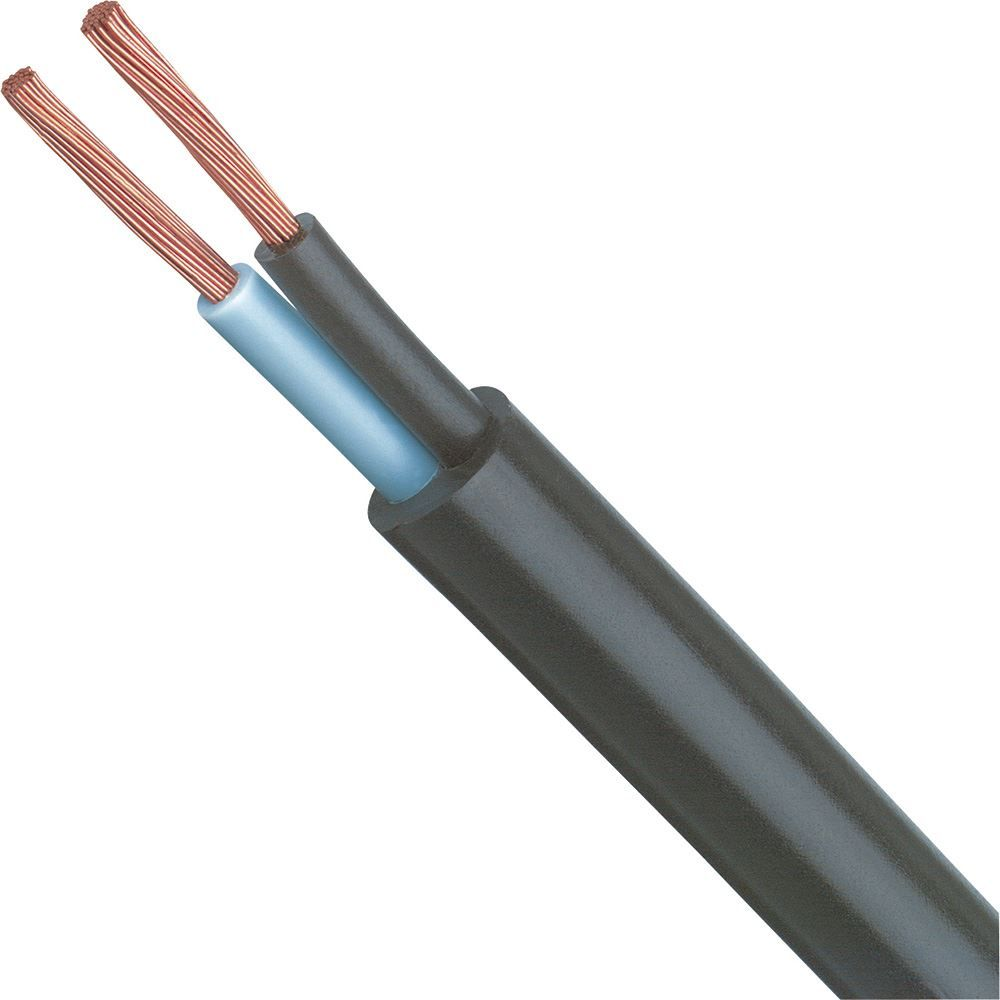
\includegraphics[keepaspectratio=true,scale=0.15] {Figuras/BASE/energiabase/cabopp.jpg}
  \caption{Cabo flexível pp 2X2,5mm² com extremidade descascada.} 
  \label{fig:cabopp}
\end{figure}
Passo 14 - Soldar a extremidade descascada do cabo preto a entrada indicada como negativa do adaptador Jack P4 macho, e a extremidade do cabo azul a entrada indicada como positiva, conforme Figura \ref{conexao_jack}. Utilizar a fita isolante para selar a conexão entre o cabo e o adaptador.

Passo 15 - Repetir o procedimento do passo 13 e passo 14 para a outra extremidade do cabo pp 2X2,5mm². Sendo assim, ambas as extremidades devem estar conectadas a um adaptador Jack P4 macho.

\subsection*{Conectores da base de lançamento}

Para conectar o ignitor, o atuador do desengate, e os dois atuadores das válvulas é necessário que os conectores na extremidade de cada cabo sejam sejam do tipo Jack P4 macho, pois os conectores disponíveis na base para o acoplamento desses cabos são do tipo Jack P4 fêmea. Repetir o passo 13 e passo 14 para a extremidade a ser conectada na base de cada um dos 4 cabos (ignitor, atuador do desengate e os dois atuadores das válvulas).
